\documentclass[a4paper]{article}
\usepackage[fleqn]{amsmath}
\usepackage{graphicx}
%\usepackage{times}
\usepackage[framed,numbered,autolinebreaks,useliterate]{mcode}
\usepackage{listing}
\usepackage[small,compact]{titlesec}
\usepackage[utf8x]{inputenc}

\usepackage[paper=a4paper,
            %includefoot, % Uncomment to put page number above margin
            marginparwidth=30.5mm,    % Length of section titles
            marginparsep=1.5mm,       % Space between titles and text
            margin=25mm,              % 25mm margins
            includemp]{geometry}


\newcommand{\makeheading}[2]%
        {\hspace*{-\marginparsep minus \marginparwidth}%
         \begin{minipage}[t]{\textwidth\marginparwidth\marginparsep}%
           {\large \bfseries #1}\\{#2}\\[-0.15\baselineskip]%
                 \rule{\columnwidth}{1pt}%
         \end{minipage}}

\newlength{\figurewidth}
\setlength{\figurewidth}{500px}
\begin{document}
\makeheading{Gautebøye, rev1, Instrument response}{Gaute Hope
(gaute.hope@student.uib.no)}

\section{Hydrophone decoupling}
\begin{figure}[h]
  \begin{center}
  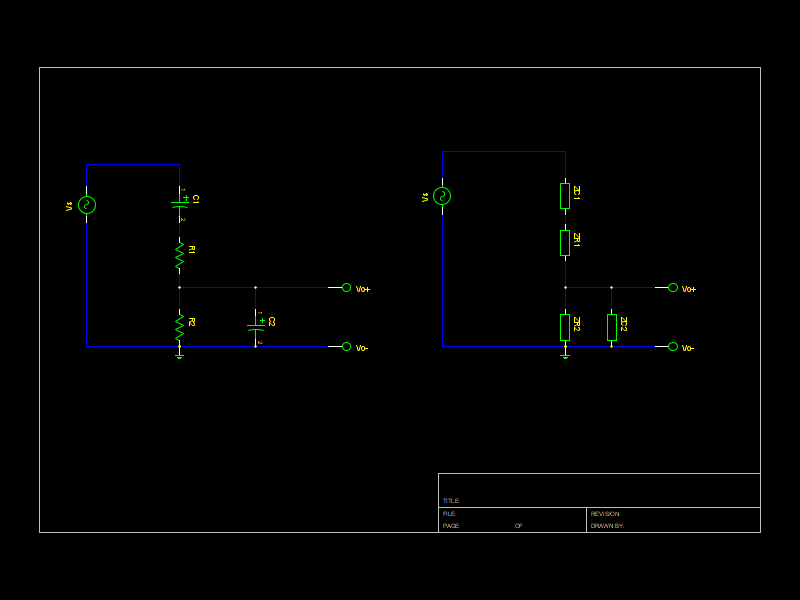
\includegraphics[width=400px]{Hydrophone_decoupling.png}
\end{center}
  \caption{Hydrophone decoupling circuit}
  \label{fig:hydrophone_decoupling}
\end{figure}

The figure above (\ref{fig:hydrophone_decoupling}) shows an equivalent
circuit of the deployed input decoupling to the hydrophone.

\paragraph{}The circuit was based on the suggested decoupling in figure
\ref{fig:suggested_decoupling} seen below, it was designed to have the
same properties, but also low-pass the signal at cutoff frequency
$f_{LP}$. The original design already decouples, and high-passes, the
signal at frequency $f_{HP}$.

\begin{figure}[h!]
  \begin{center}
    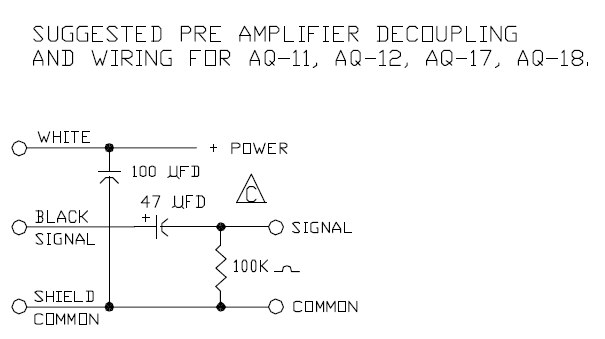
\includegraphics[width=200px]{AQ-18-decoupling-and-wiring.jpg}
  \end{center}
  \caption{AQ-18 suggested decoupling and wiring}
  \label{fig:suggested_decoupling}
\end{figure}

\section{Derivation of transfer function}

$i_1$ and $i_2$ signify the current loops passing through respectively left
and right loop. Using Kirchoff's equation:

\begin{align}
  \label{eqn:currents_1}
  V_s &= i_1 (Z_{C_1} + Z_{R_1}) + (i_1 - i_2) \cdot Z_{R_2} \\
  0   &= (i_2 - i_1) \cdot Z_{R_2} + i_2 \cdot Z_{C_2}
  \label{eqn:currents_2}
\end{align}

$V_s$ is the signal source, the hydrophone. See separate data sheet for
hydrophone frequency response. $V_o$, output, is measured at the
terminals $T_+$ and $T_-$.

\begin{align}
  \label{eqn:vo}
  V_o &= i_2 \cdot Z_{C_2} \\
  H(s) &= \frac{V_o}{V_s}, s = i\omega
\end{align}

Solving for $H(s)$ gives:

\begin{equation}
  H(s) = \frac{8.218 \cdot 10^{60} \times s^2}
  {1.822 \cdot 10^{56} \times s^3 +
   1.972 \cdot 10^{61} \times s^2 +
   4.196 \cdot 10^{60} \times s}
  \label{eqn:transferfunction}
\end{equation}

A bode plot of the transfer function (instrument response) is shown in
figure \ref{fig:bodeplot} below.
\begin{figure}[h!]
  \begin{center}
    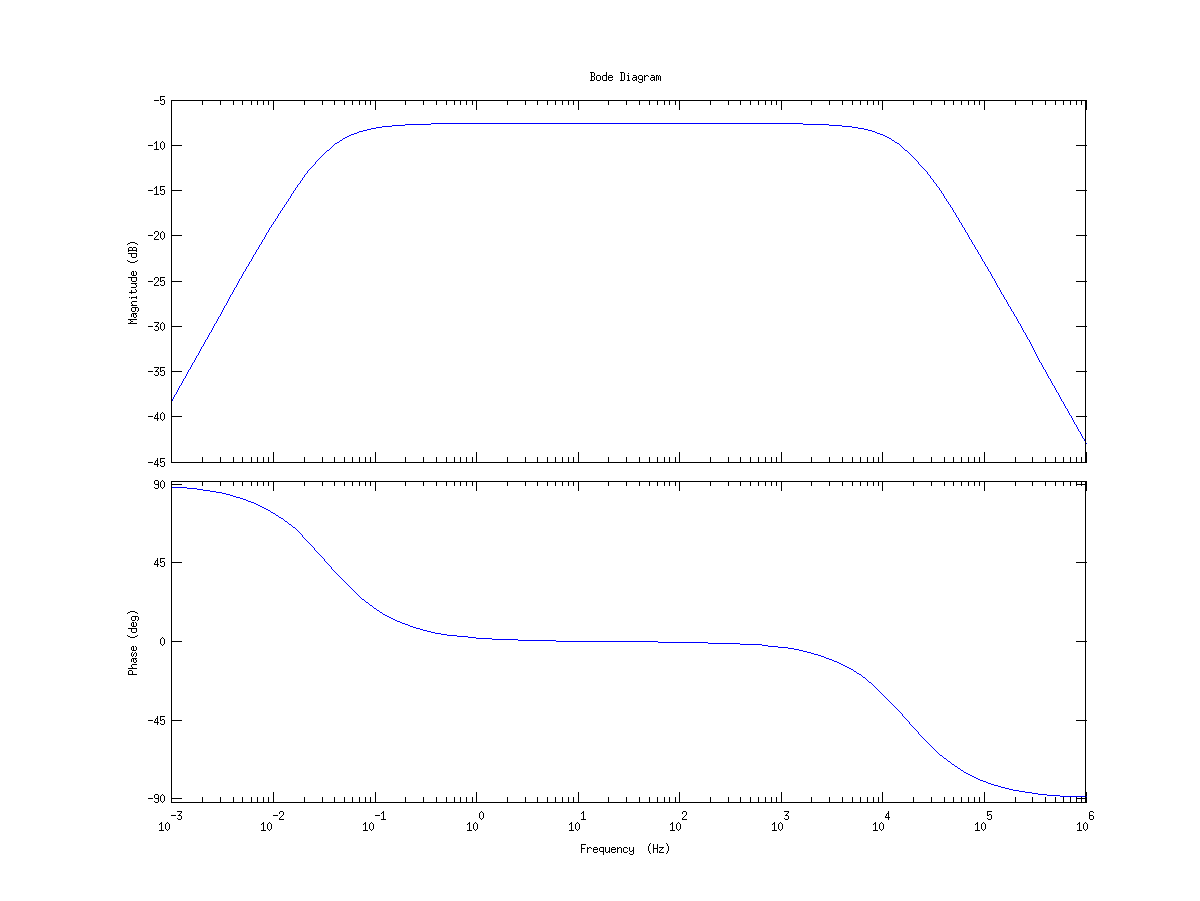
\includegraphics[width=400px]{bodeplot.png}
  \end{center}
  \caption{Bode plot of transfer function}
  \label{fig:bodeplot}
\end{figure}

Equation \ref{eqn:transferfunction} can be solved by using the MATLAB
script response.m, the Bode plot in figure \ref{fig:bodeplot} was
created with the same script.
\newpage
\section{response.m}
\lstinputlisting{response.m}


\end{document}

